\documentclass[11pt,a4paper]{article}
\usepackage[margin=2.5cm]{geometry}
\usepackage{setspace}
\usepackage{hyperref}
\usepackage{amsmath}
\usepackage{float}
\usepackage{graphicx}
\setstretch{1.15}
\usepackage[utf8]{inputenc}
\title{Mode Connectivity in Neural Networks}
\author{Maciek Lodzinski}
\date{January 27th 2026}
\begin{document}
\maketitle

\section{Observations on Loss Curve Characteristics}

\begin{figure}[H]
    \centering
    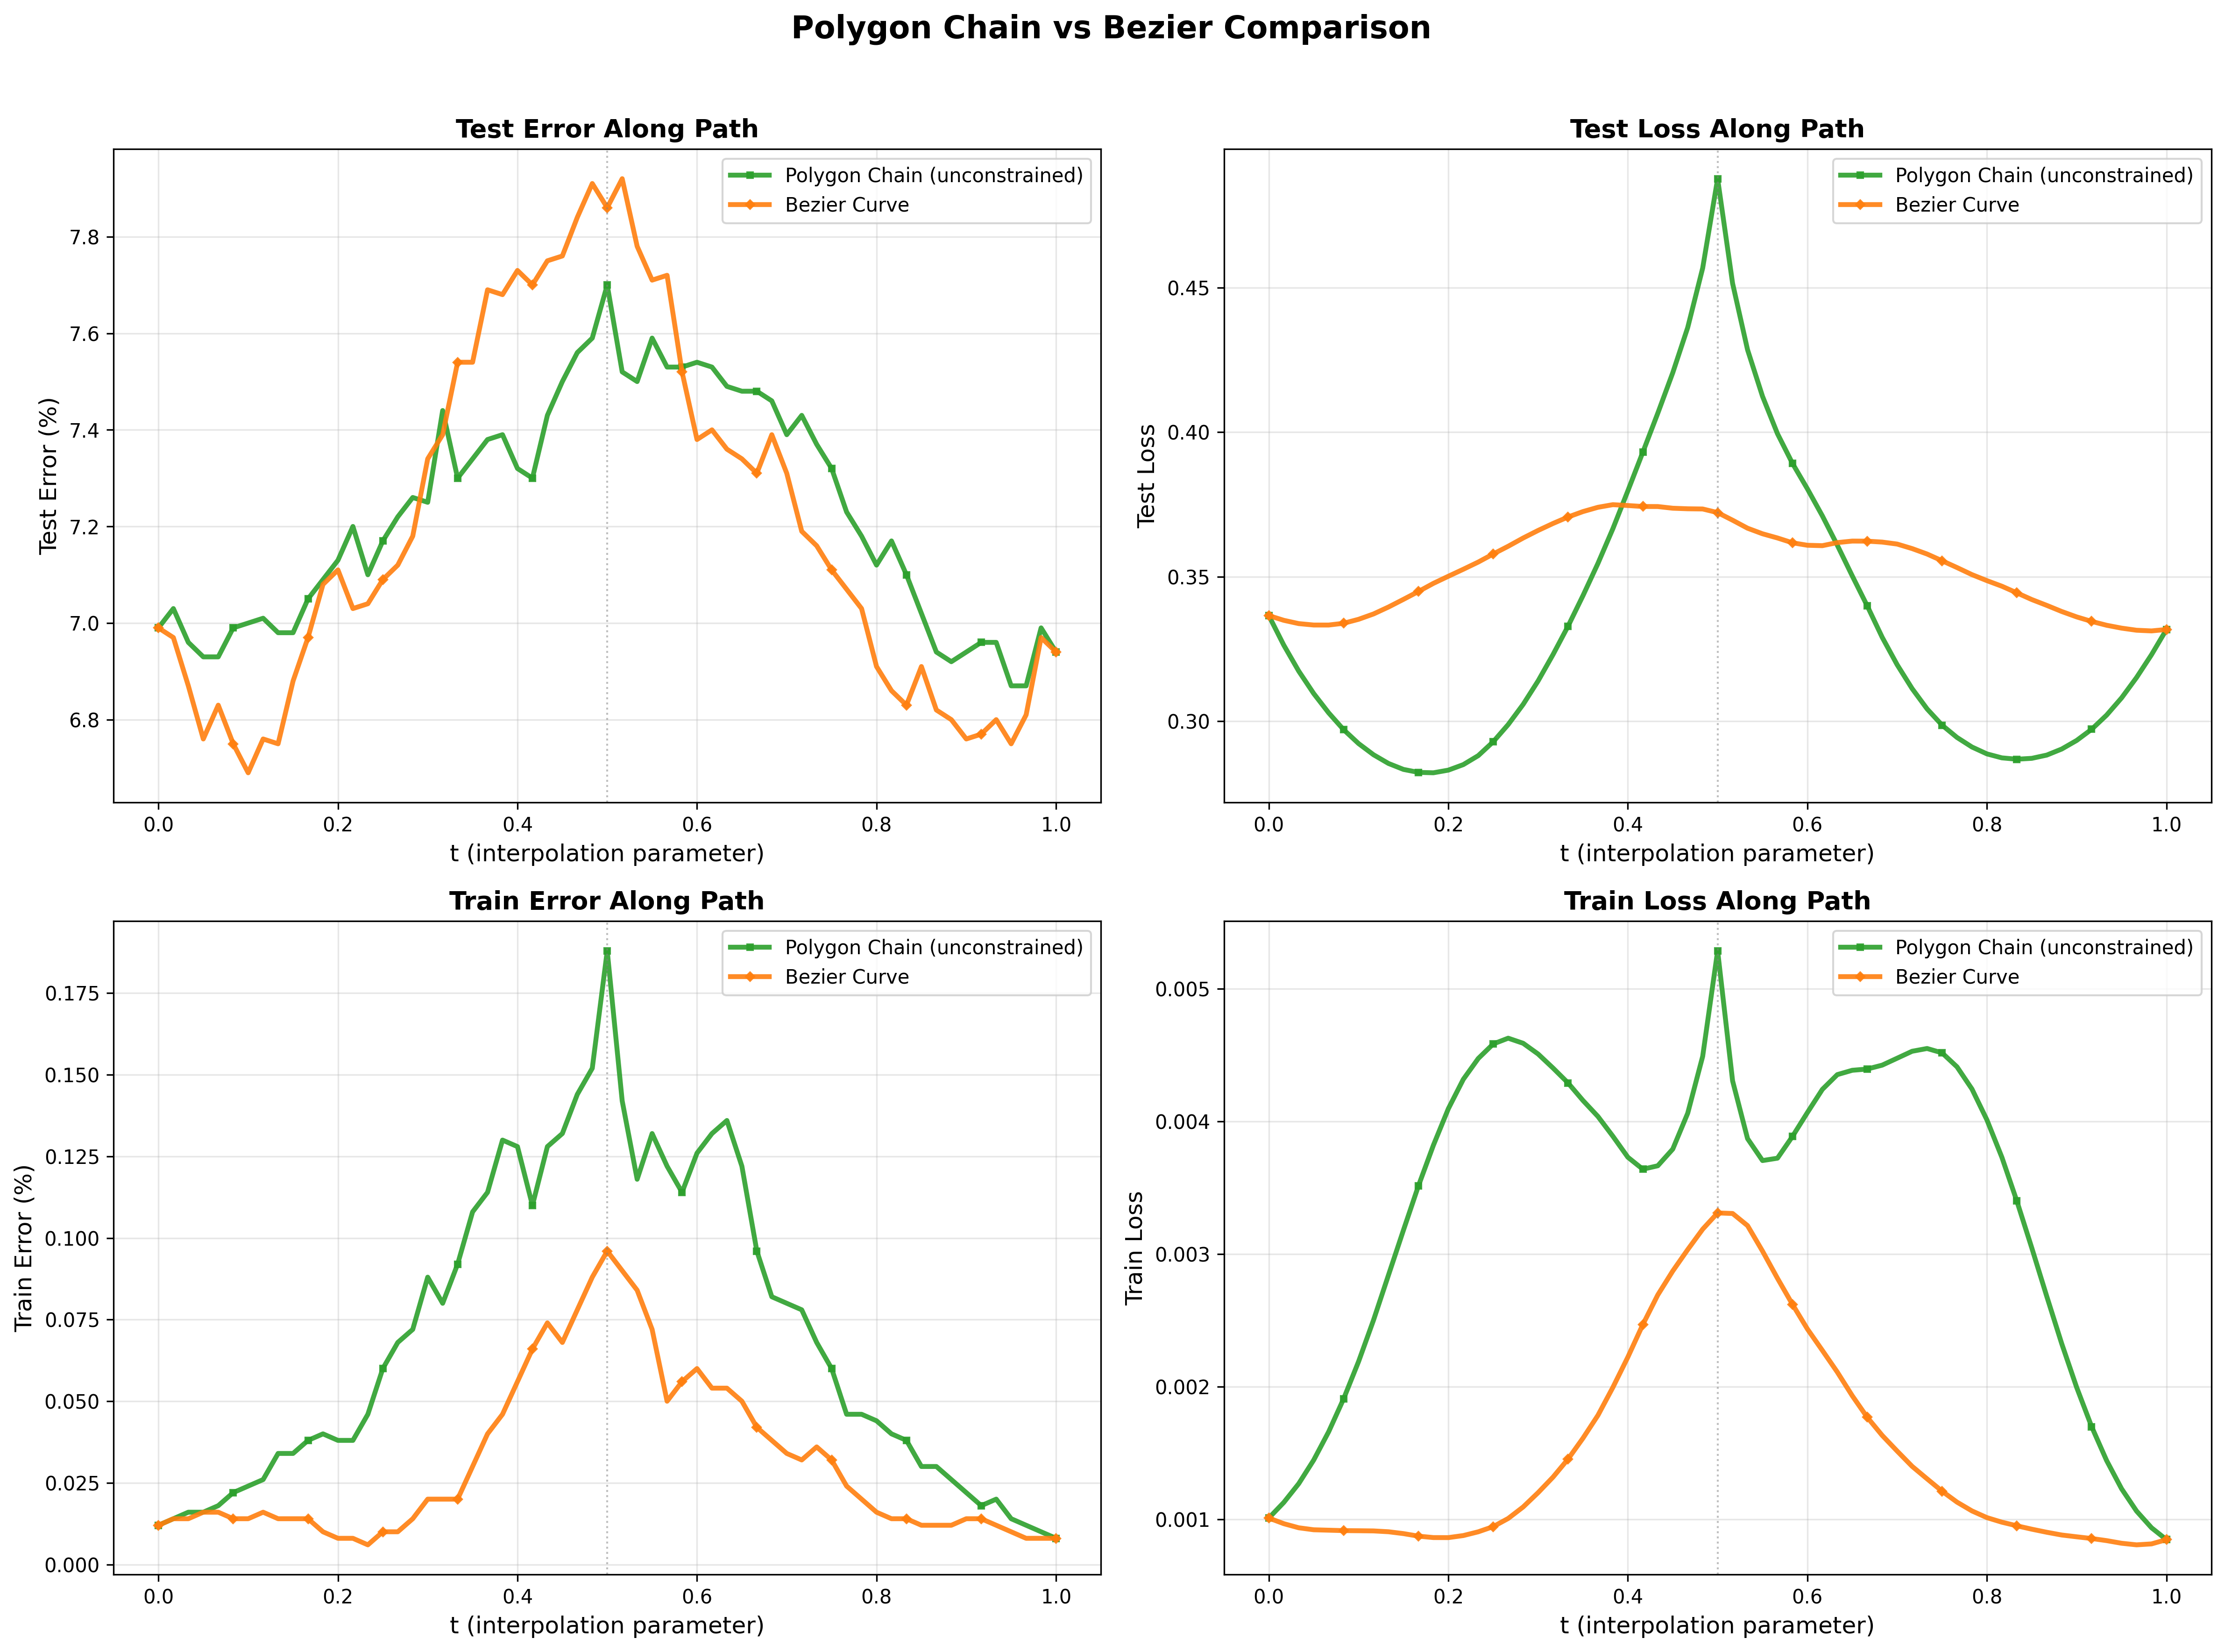
\includegraphics[width=1\linewidth]{example.png}
    \caption{VGG16 on CIFAR-10, without train augmentations}
    \label{fig:placeholder}
\end{figure}

Through code analysis and verification experiments, several important observations emerged regarding the loss and accuracy curves along connectivity paths:

\textbf{Curve Smoothness:} Under standard evaluation conditions (without random augmentations), the loss curves exhibit very smooth, continuous behavior. Initial apparent noise in some curves was traced to those random data augmentations (horizontal flips, random crops) being applied during evaluation on the training split. This was corrected to ensure consistent evaluation conditions.
\newpage
\begin{figure}[H]
    \centering
    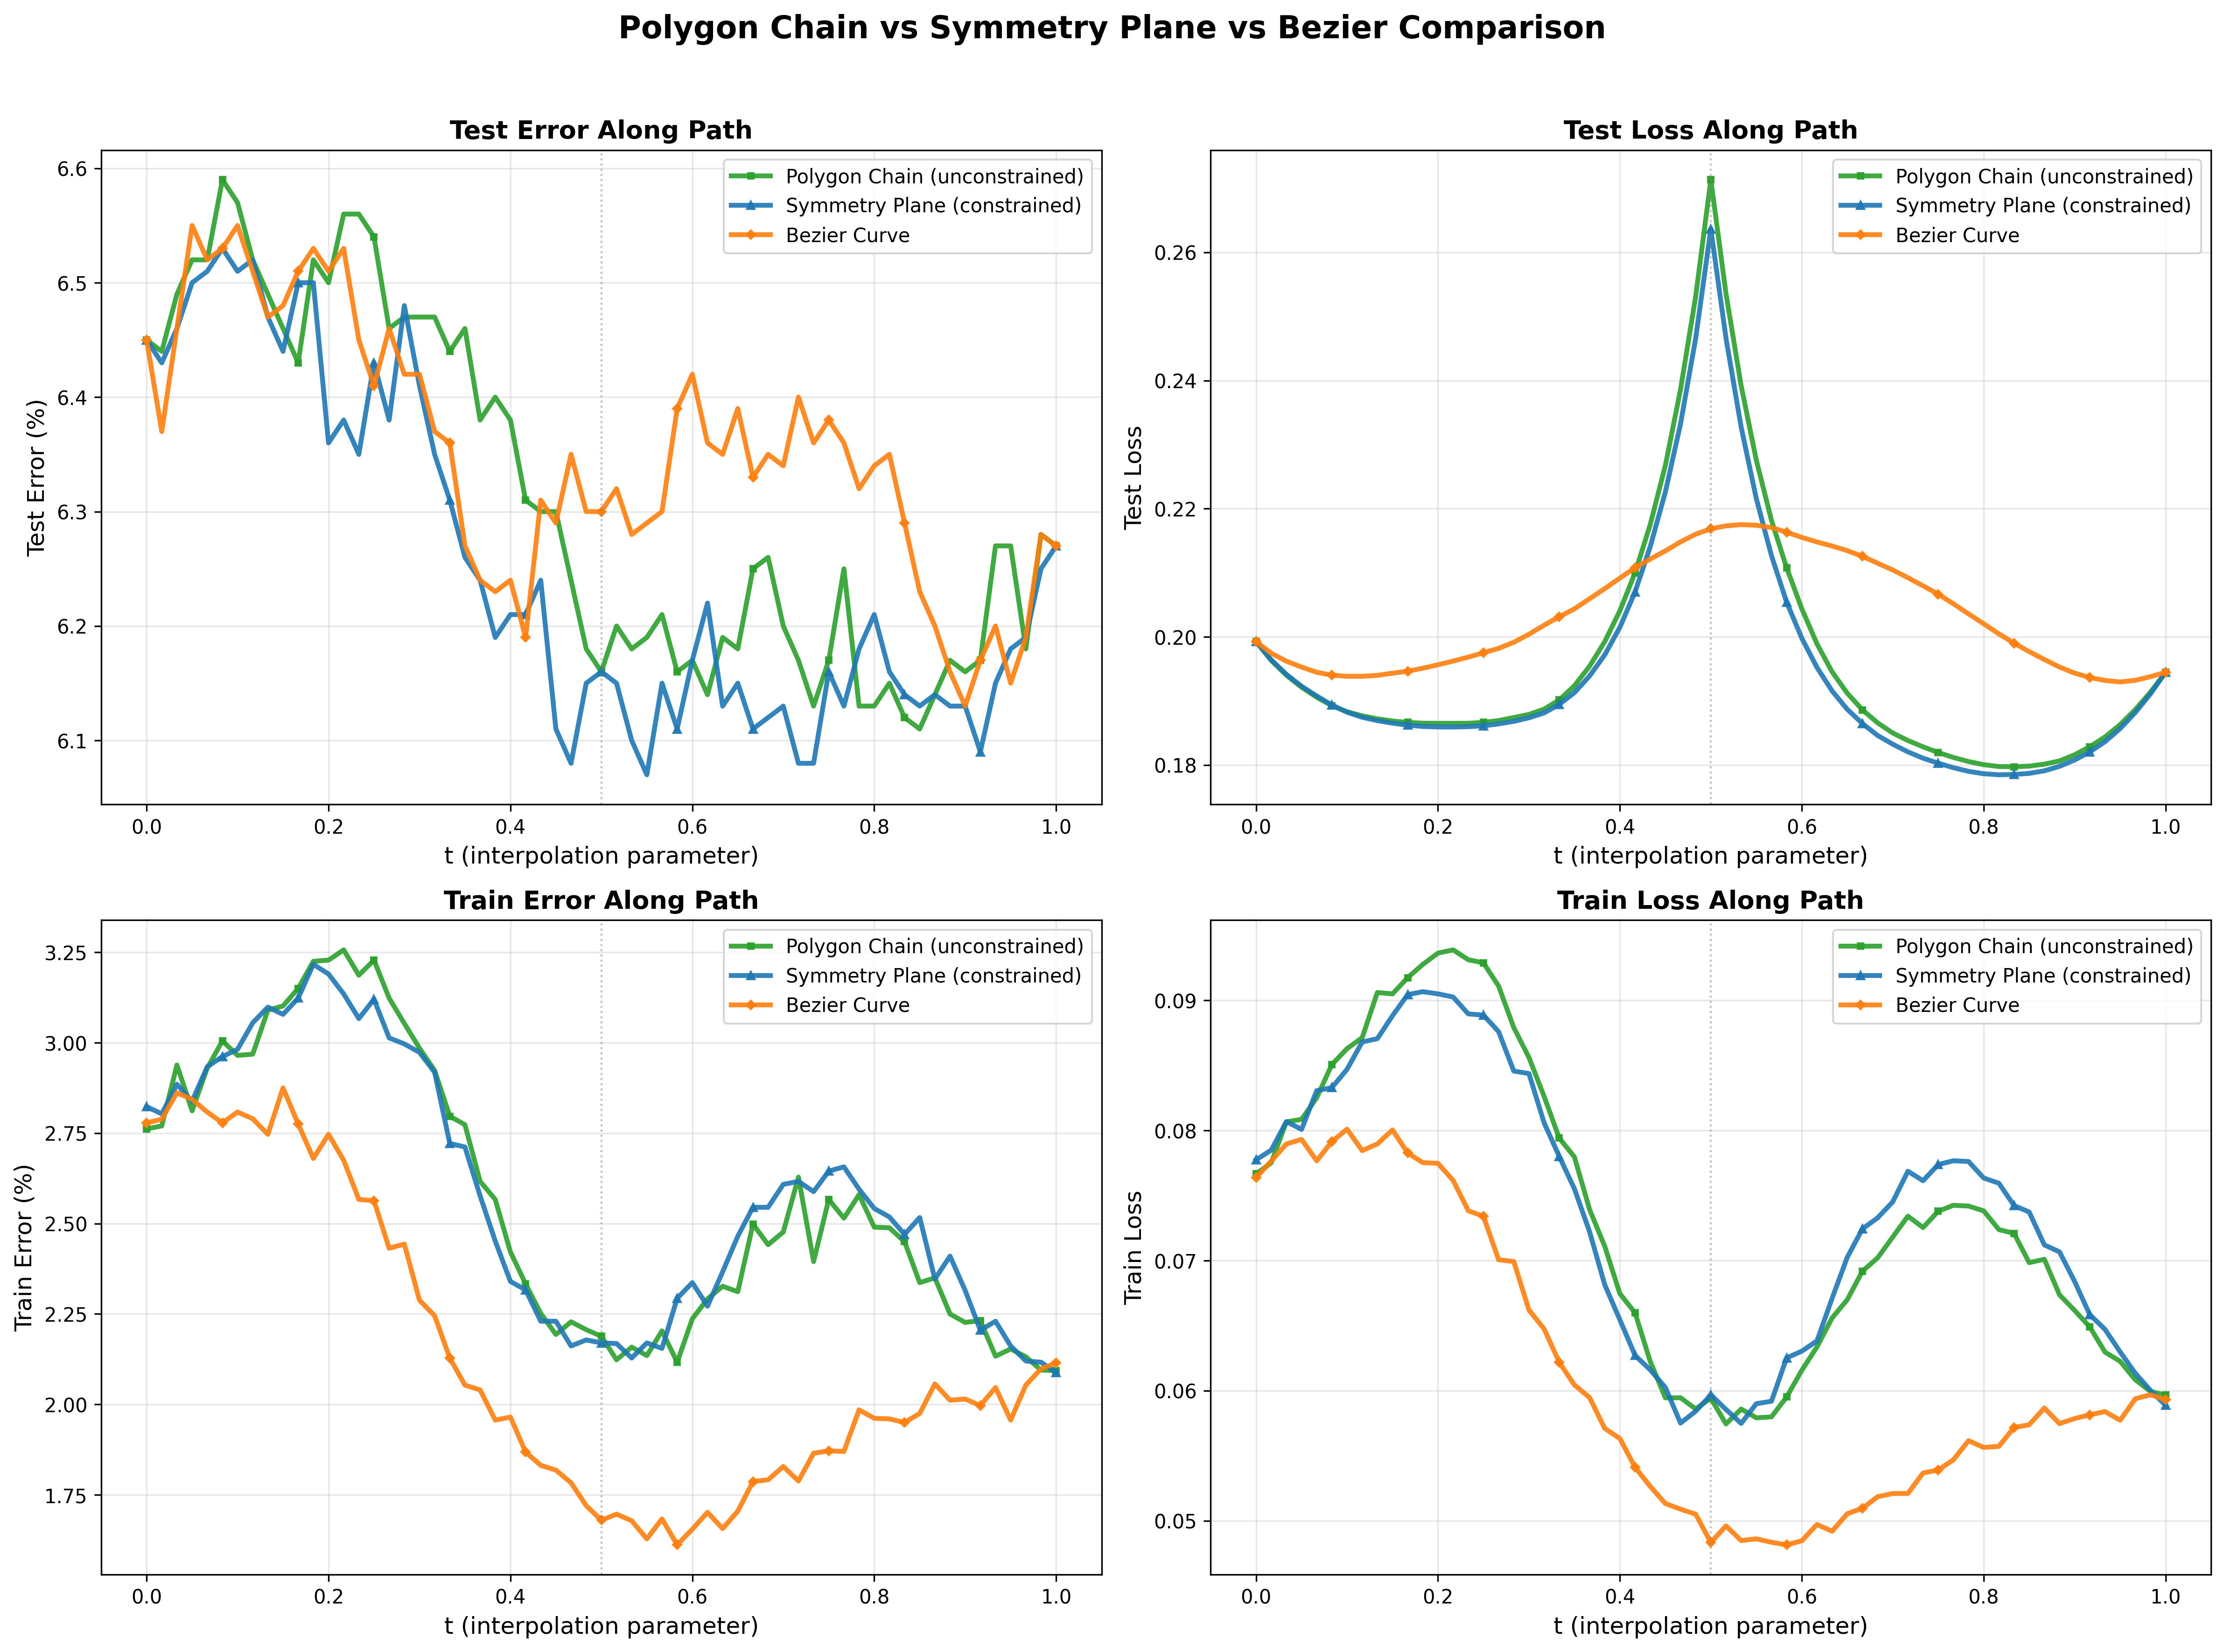
\includegraphics[width=1\linewidth]{example_2.png}
    \caption{CONVFC on FMNIST, with train augmentations}
    \label{fig:placeholder}
\end{figure}
\textbf{Train vs.\ Test Loss Differences:} The apparent differences between train and test loss curves are correct from what I understand. In both VGG16 on CIFAR-10 and ConvFC on Fashion-MNIST, the models exhibited overfitting on the training data. Consequently, the train loss curves appear nearly flat along the connectivity path when plotted on the same scale as test loss curves. This does not indicate different data distributions or evaluation errors. The test loss curves, evaluating on unseen data, naturally show higher values and more pronounced variation along the path.

\textbf{Endpoint Consistency:} Initial observations showed that loss and accuracy values at the endpoints ($t=0$ and $t=1.0$) varied slightly across different path-finding methods. This variation was also attributed to random augmentations being applied during batch normalization statistics updates on the training split. When augmentations were disabled for evaluation, endpoint values became consistent across all methods, as expected.\\

\textbf{Conclusion}

\begin{itemize}
    \item The trained path at $t = 0.5$ demonstrates improved fitting to the training data, as indicated by a reduced training loss (CONVFC on MNIST). Notably, the low-loss path-finding methods employ the same regularization as both endpoint models; nevertheless, the intermediate solution attains a lower training-loss minimum while exhibiting degraded generalization performance. This suggests that factors such as differing initialization or optimization dynamics may enable these methods to converge to sharper minima that favor training performance at the expense of test performance.
    \item This improvement comes at the expense of generalization performance, reflected by an increase in test loss.
    \item At approximately $93\%$ accuracy, most remaining classification errors are primarily attributable to inherently ambiguous samples and label noise (there are known mislabeled samples in CIFAR10 and FMNIST). Consequently, further model improvements tend to sharpen confidence on already-correct predictions rather than substantially modifying decision boundaries. This behavior is evident when comparing the training and test losses at $t = 0.2$ and $t = 0.5$, where a loss difference of approximately $0.2$ corresponds to only a $0.8\%$ difference in classification accuracy.

\end{itemize}

\begin{figure}[htbp]
    \centering
    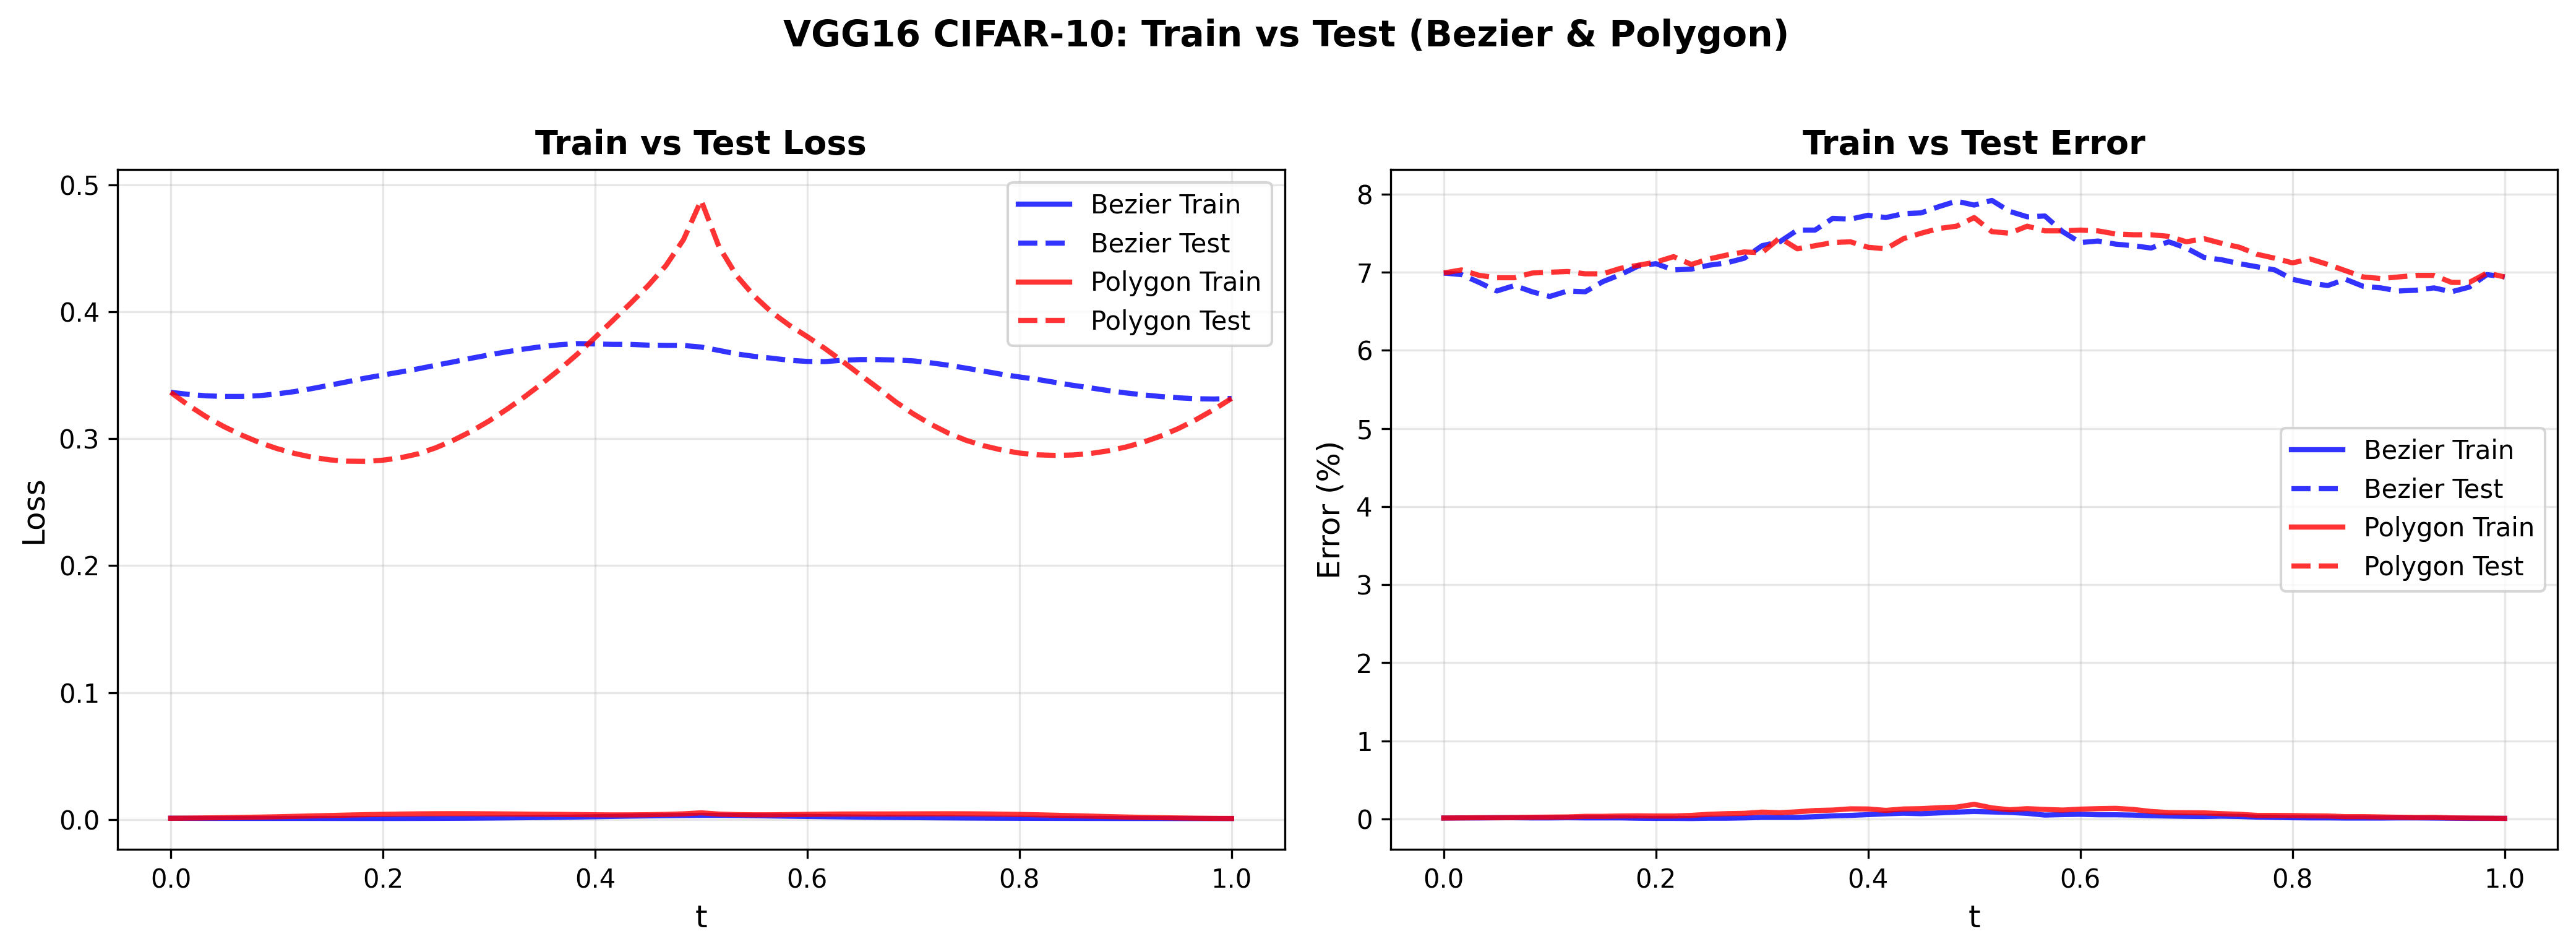
\includegraphics[width=1.1\linewidth]{vgg16.png}\\[0.5em]
    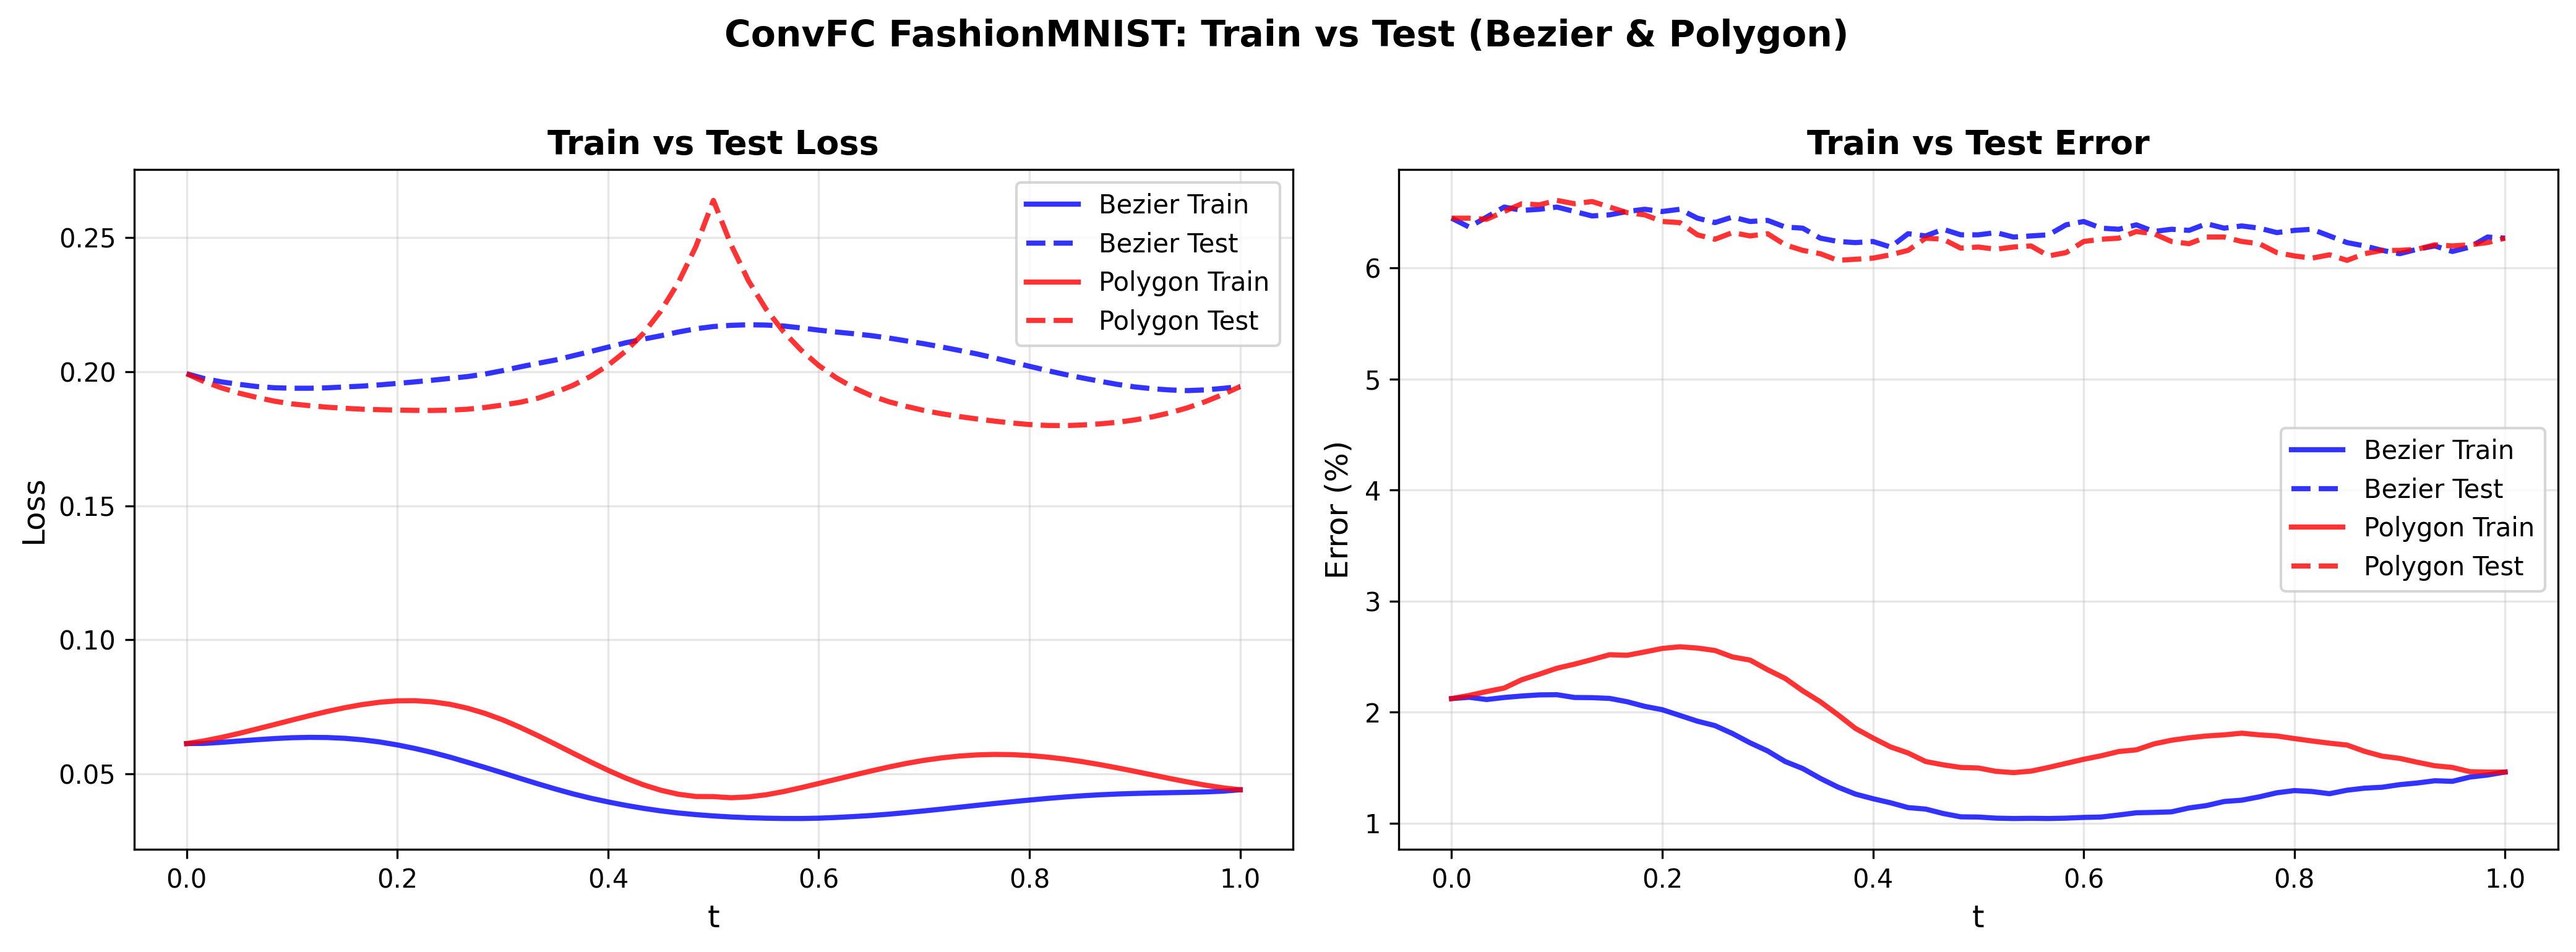
\includegraphics[width=1.1\linewidth]{convfc.png}
    \caption{Comparison of VGG16 architecture and Conv+FC architecture}
    \label{fig:vgg16_convfc}
\end{figure}   


\end{document}